% Options for packages loaded elsewhere
\PassOptionsToPackage{unicode}{hyperref}
\PassOptionsToPackage{hyphens}{url}
\PassOptionsToPackage{dvipsnames,svgnames,x11names}{xcolor}
%
\documentclass[
  letterpaper,
  DIV=11,
  numbers=noendperiod]{scrartcl}

\usepackage{amsmath,amssymb}
\usepackage{iftex}
\ifPDFTeX
  \usepackage[T1]{fontenc}
  \usepackage[utf8]{inputenc}
  \usepackage{textcomp} % provide euro and other symbols
\else % if luatex or xetex
  \usepackage{unicode-math}
  \defaultfontfeatures{Scale=MatchLowercase}
  \defaultfontfeatures[\rmfamily]{Ligatures=TeX,Scale=1}
\fi
\usepackage{lmodern}
\ifPDFTeX\else  
    % xetex/luatex font selection
\fi
% Use upquote if available, for straight quotes in verbatim environments
\IfFileExists{upquote.sty}{\usepackage{upquote}}{}
\IfFileExists{microtype.sty}{% use microtype if available
  \usepackage[]{microtype}
  \UseMicrotypeSet[protrusion]{basicmath} % disable protrusion for tt fonts
}{}
\makeatletter
\@ifundefined{KOMAClassName}{% if non-KOMA class
  \IfFileExists{parskip.sty}{%
    \usepackage{parskip}
  }{% else
    \setlength{\parindent}{0pt}
    \setlength{\parskip}{6pt plus 2pt minus 1pt}}
}{% if KOMA class
  \KOMAoptions{parskip=half}}
\makeatother
\usepackage{xcolor}
\setlength{\emergencystretch}{3em} % prevent overfull lines
\setcounter{secnumdepth}{-\maxdimen} % remove section numbering
% Make \paragraph and \subparagraph free-standing
\makeatletter
\ifx\paragraph\undefined\else
  \let\oldparagraph\paragraph
  \renewcommand{\paragraph}{
    \@ifstar
      \xxxParagraphStar
      \xxxParagraphNoStar
  }
  \newcommand{\xxxParagraphStar}[1]{\oldparagraph*{#1}\mbox{}}
  \newcommand{\xxxParagraphNoStar}[1]{\oldparagraph{#1}\mbox{}}
\fi
\ifx\subparagraph\undefined\else
  \let\oldsubparagraph\subparagraph
  \renewcommand{\subparagraph}{
    \@ifstar
      \xxxSubParagraphStar
      \xxxSubParagraphNoStar
  }
  \newcommand{\xxxSubParagraphStar}[1]{\oldsubparagraph*{#1}\mbox{}}
  \newcommand{\xxxSubParagraphNoStar}[1]{\oldsubparagraph{#1}\mbox{}}
\fi
\makeatother

\usepackage{color}
\usepackage{fancyvrb}
\newcommand{\VerbBar}{|}
\newcommand{\VERB}{\Verb[commandchars=\\\{\}]}
\DefineVerbatimEnvironment{Highlighting}{Verbatim}{commandchars=\\\{\}}
% Add ',fontsize=\small' for more characters per line
\usepackage{framed}
\definecolor{shadecolor}{RGB}{241,243,245}
\newenvironment{Shaded}{\begin{snugshade}}{\end{snugshade}}
\newcommand{\AlertTok}[1]{\textcolor[rgb]{0.68,0.00,0.00}{#1}}
\newcommand{\AnnotationTok}[1]{\textcolor[rgb]{0.37,0.37,0.37}{#1}}
\newcommand{\AttributeTok}[1]{\textcolor[rgb]{0.40,0.45,0.13}{#1}}
\newcommand{\BaseNTok}[1]{\textcolor[rgb]{0.68,0.00,0.00}{#1}}
\newcommand{\BuiltInTok}[1]{\textcolor[rgb]{0.00,0.23,0.31}{#1}}
\newcommand{\CharTok}[1]{\textcolor[rgb]{0.13,0.47,0.30}{#1}}
\newcommand{\CommentTok}[1]{\textcolor[rgb]{0.37,0.37,0.37}{#1}}
\newcommand{\CommentVarTok}[1]{\textcolor[rgb]{0.37,0.37,0.37}{\textit{#1}}}
\newcommand{\ConstantTok}[1]{\textcolor[rgb]{0.56,0.35,0.01}{#1}}
\newcommand{\ControlFlowTok}[1]{\textcolor[rgb]{0.00,0.23,0.31}{\textbf{#1}}}
\newcommand{\DataTypeTok}[1]{\textcolor[rgb]{0.68,0.00,0.00}{#1}}
\newcommand{\DecValTok}[1]{\textcolor[rgb]{0.68,0.00,0.00}{#1}}
\newcommand{\DocumentationTok}[1]{\textcolor[rgb]{0.37,0.37,0.37}{\textit{#1}}}
\newcommand{\ErrorTok}[1]{\textcolor[rgb]{0.68,0.00,0.00}{#1}}
\newcommand{\ExtensionTok}[1]{\textcolor[rgb]{0.00,0.23,0.31}{#1}}
\newcommand{\FloatTok}[1]{\textcolor[rgb]{0.68,0.00,0.00}{#1}}
\newcommand{\FunctionTok}[1]{\textcolor[rgb]{0.28,0.35,0.67}{#1}}
\newcommand{\ImportTok}[1]{\textcolor[rgb]{0.00,0.46,0.62}{#1}}
\newcommand{\InformationTok}[1]{\textcolor[rgb]{0.37,0.37,0.37}{#1}}
\newcommand{\KeywordTok}[1]{\textcolor[rgb]{0.00,0.23,0.31}{\textbf{#1}}}
\newcommand{\NormalTok}[1]{\textcolor[rgb]{0.00,0.23,0.31}{#1}}
\newcommand{\OperatorTok}[1]{\textcolor[rgb]{0.37,0.37,0.37}{#1}}
\newcommand{\OtherTok}[1]{\textcolor[rgb]{0.00,0.23,0.31}{#1}}
\newcommand{\PreprocessorTok}[1]{\textcolor[rgb]{0.68,0.00,0.00}{#1}}
\newcommand{\RegionMarkerTok}[1]{\textcolor[rgb]{0.00,0.23,0.31}{#1}}
\newcommand{\SpecialCharTok}[1]{\textcolor[rgb]{0.37,0.37,0.37}{#1}}
\newcommand{\SpecialStringTok}[1]{\textcolor[rgb]{0.13,0.47,0.30}{#1}}
\newcommand{\StringTok}[1]{\textcolor[rgb]{0.13,0.47,0.30}{#1}}
\newcommand{\VariableTok}[1]{\textcolor[rgb]{0.07,0.07,0.07}{#1}}
\newcommand{\VerbatimStringTok}[1]{\textcolor[rgb]{0.13,0.47,0.30}{#1}}
\newcommand{\WarningTok}[1]{\textcolor[rgb]{0.37,0.37,0.37}{\textit{#1}}}

\providecommand{\tightlist}{%
  \setlength{\itemsep}{0pt}\setlength{\parskip}{0pt}}\usepackage{longtable,booktabs,array}
\usepackage{calc} % for calculating minipage widths
% Correct order of tables after \paragraph or \subparagraph
\usepackage{etoolbox}
\makeatletter
\patchcmd\longtable{\par}{\if@noskipsec\mbox{}\fi\par}{}{}
\makeatother
% Allow footnotes in longtable head/foot
\IfFileExists{footnotehyper.sty}{\usepackage{footnotehyper}}{\usepackage{footnote}}
\makesavenoteenv{longtable}
\usepackage{graphicx}
\makeatletter
\def\maxwidth{\ifdim\Gin@nat@width>\linewidth\linewidth\else\Gin@nat@width\fi}
\def\maxheight{\ifdim\Gin@nat@height>\textheight\textheight\else\Gin@nat@height\fi}
\makeatother
% Scale images if necessary, so that they will not overflow the page
% margins by default, and it is still possible to overwrite the defaults
% using explicit options in \includegraphics[width, height, ...]{}
\setkeys{Gin}{width=\maxwidth,height=\maxheight,keepaspectratio}
% Set default figure placement to htbp
\makeatletter
\def\fps@figure{htbp}
\makeatother

\KOMAoption{captions}{tableheading}
\makeatletter
\@ifpackageloaded{caption}{}{\usepackage{caption}}
\AtBeginDocument{%
\ifdefined\contentsname
  \renewcommand*\contentsname{Table of contents}
\else
  \newcommand\contentsname{Table of contents}
\fi
\ifdefined\listfigurename
  \renewcommand*\listfigurename{List of Figures}
\else
  \newcommand\listfigurename{List of Figures}
\fi
\ifdefined\listtablename
  \renewcommand*\listtablename{List of Tables}
\else
  \newcommand\listtablename{List of Tables}
\fi
\ifdefined\figurename
  \renewcommand*\figurename{Figure}
\else
  \newcommand\figurename{Figure}
\fi
\ifdefined\tablename
  \renewcommand*\tablename{Table}
\else
  \newcommand\tablename{Table}
\fi
}
\@ifpackageloaded{float}{}{\usepackage{float}}
\floatstyle{ruled}
\@ifundefined{c@chapter}{\newfloat{codelisting}{h}{lop}}{\newfloat{codelisting}{h}{lop}[chapter]}
\floatname{codelisting}{Listing}
\newcommand*\listoflistings{\listof{codelisting}{List of Listings}}
\makeatother
\makeatletter
\makeatother
\makeatletter
\@ifpackageloaded{caption}{}{\usepackage{caption}}
\@ifpackageloaded{subcaption}{}{\usepackage{subcaption}}
\makeatother

\ifLuaTeX
  \usepackage{selnolig}  % disable illegal ligatures
\fi
\usepackage{bookmark}

\IfFileExists{xurl.sty}{\usepackage{xurl}}{} % add URL line breaks if available
\urlstyle{same} % disable monospaced font for URLs
\hypersetup{
  pdftitle={proj data},
  colorlinks=true,
  linkcolor={blue},
  filecolor={Maroon},
  citecolor={Blue},
  urlcolor={Blue},
  pdfcreator={LaTeX via pandoc}}


\title{proj data}
\author{}
\date{}

\begin{document}
\maketitle


\subsection{Quarto}\label{quarto}

Quarto enables you to weave together content and executable code into a
finished document. To learn more about Quarto see
\url{https://quarto.org}.

\subsection{Running Code}\label{running-code}

When you click the \textbf{Render} button a document will be generated
that includes both content and the output of embedded code. You can
embed code like this:

\begin{Shaded}
\begin{Highlighting}[]
\FunctionTok{library}\NormalTok{(tidyverse)}
\end{Highlighting}
\end{Shaded}

\begin{verbatim}
-- Attaching core tidyverse packages ------------------------ tidyverse 2.0.0 --
v dplyr     1.1.4     v readr     2.1.5
v forcats   1.0.0     v stringr   1.5.1
v ggplot2   3.5.1     v tibble    3.2.1
v lubridate 1.9.3     v tidyr     1.3.1
v purrr     1.0.2     
-- Conflicts ------------------------------------------ tidyverse_conflicts() --
x dplyr::filter() masks stats::filter()
x dplyr::lag()    masks stats::lag()
i Use the conflicted package (<http://conflicted.r-lib.org/>) to force all conflicts to become errors
\end{verbatim}

\begin{Shaded}
\begin{Highlighting}[]
\FunctionTok{library}\NormalTok{(ggplot2)}
\end{Highlighting}
\end{Shaded}

\begin{Shaded}
\begin{Highlighting}[]
\NormalTok{depression }\OtherTok{\textless{}{-}} \FunctionTok{read.csv}\NormalTok{(}\StringTok{"Depression Student Dataset.csv"}\NormalTok{)}
\end{Highlighting}
\end{Shaded}

You can add options to executable code like this

\begin{Shaded}
\begin{Highlighting}[]
\NormalTok{depression\_age }\OtherTok{\textless{}{-}}\NormalTok{ depression }\SpecialCharTok{\%\textgreater{}\%} \FunctionTok{group\_by}\NormalTok{(Gender, Age, Depression) }\SpecialCharTok{\%\textgreater{}\%} \FunctionTok{summarise}\NormalTok{(}\AttributeTok{count=}\FunctionTok{n}\NormalTok{())}
\end{Highlighting}
\end{Shaded}

\begin{verbatim}
`summarise()` has grouped output by 'Gender', 'Age'. You can override using the
`.groups` argument.
\end{verbatim}

\begin{Shaded}
\begin{Highlighting}[]
\NormalTok{are\_d }\OtherTok{\textless{}{-}}\NormalTok{ depression\_age }\SpecialCharTok{\%\textgreater{}\%} \FunctionTok{filter}\NormalTok{(Depression }\SpecialCharTok{==} \StringTok{"Yes"}\NormalTok{)}
\NormalTok{are\_nd }\OtherTok{\textless{}{-}}\NormalTok{ depression\_age }\SpecialCharTok{\%\textgreater{}\%} \FunctionTok{filter}\NormalTok{(Depression }\SpecialCharTok{==} \StringTok{"No"}\NormalTok{)}

\FunctionTok{ggplot}\NormalTok{(are\_d, }\FunctionTok{aes}\NormalTok{(}\AttributeTok{x =}\NormalTok{ Age, }\AttributeTok{y =}\NormalTok{ count, }\AttributeTok{color =}\NormalTok{ Gender)) }\SpecialCharTok{+}
  \FunctionTok{geom\_point}\NormalTok{(}\AttributeTok{size =} \DecValTok{3}\NormalTok{) }\SpecialCharTok{+}    
  \FunctionTok{geom\_line}\NormalTok{() }\SpecialCharTok{+}       
  \FunctionTok{labs}\NormalTok{(}
    \AttributeTok{title =} \StringTok{"Age of Depressed Students"}\NormalTok{,}
    \AttributeTok{x =} \StringTok{"Age"}\NormalTok{,}
    \AttributeTok{y =} \StringTok{"Total"}\NormalTok{,}
    \AttributeTok{color =} \StringTok{"Gender"}
\NormalTok{  ) }\SpecialCharTok{+}
  \FunctionTok{theme\_minimal}\NormalTok{() }
\end{Highlighting}
\end{Shaded}

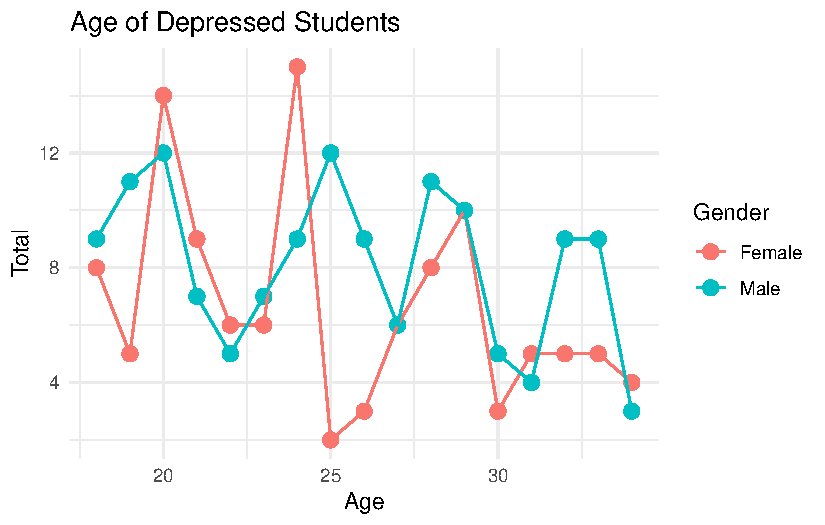
\includegraphics{Data_files/figure-pdf/unnamed-chunk-3-1.pdf}

\begin{Shaded}
\begin{Highlighting}[]
\FunctionTok{ggplot}\NormalTok{(are\_nd, }\FunctionTok{aes}\NormalTok{(}\AttributeTok{x =}\NormalTok{ Age, }\AttributeTok{y =}\NormalTok{ count, }\AttributeTok{color =}\NormalTok{ Gender)) }\SpecialCharTok{+}
  \FunctionTok{geom\_point}\NormalTok{(}\AttributeTok{size =} \DecValTok{3}\NormalTok{) }\SpecialCharTok{+}    
  \FunctionTok{geom\_line}\NormalTok{() }\SpecialCharTok{+}       
  \FunctionTok{labs}\NormalTok{(}
    \AttributeTok{title =} \StringTok{"Age of Not Depressed Students"}\NormalTok{,}
    \AttributeTok{x =} \StringTok{"Age"}\NormalTok{,}
    \AttributeTok{y =} \StringTok{"Total"}\NormalTok{,}
    \AttributeTok{color =} \StringTok{"Gender"}
\NormalTok{  ) }\SpecialCharTok{+}
  \FunctionTok{theme\_minimal}\NormalTok{() }
\end{Highlighting}
\end{Shaded}

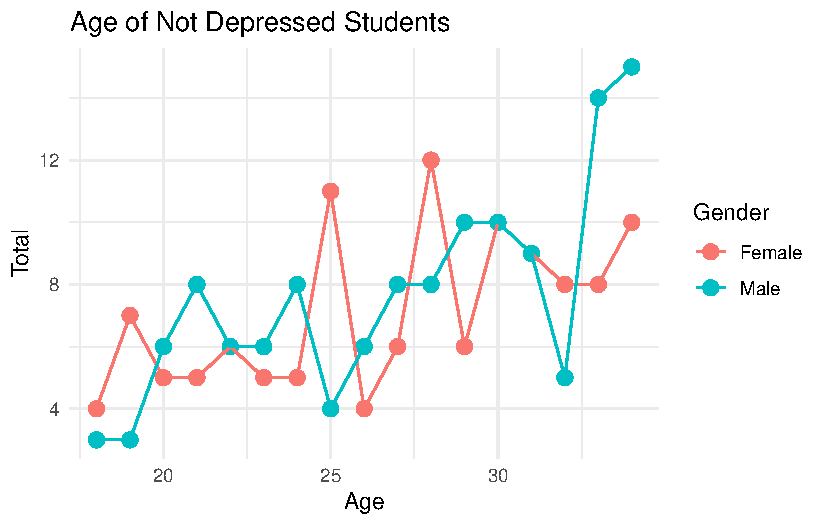
\includegraphics{Data_files/figure-pdf/unnamed-chunk-3-2.pdf}

\begin{Shaded}
\begin{Highlighting}[]
\NormalTok{depression\_press }\OtherTok{\textless{}{-}}\NormalTok{ depression }\SpecialCharTok{\%\textgreater{}\%} \FunctionTok{group\_by}\NormalTok{(Gender, Academic.Pressure, Depression) }\SpecialCharTok{\%\textgreater{}\%} \FunctionTok{summarise}\NormalTok{(}\AttributeTok{count=}\FunctionTok{n}\NormalTok{())}
\end{Highlighting}
\end{Shaded}

\begin{verbatim}
`summarise()` has grouped output by 'Gender', 'Academic.Pressure'. You can
override using the `.groups` argument.
\end{verbatim}

\begin{Shaded}
\begin{Highlighting}[]
\NormalTok{are\_d }\OtherTok{\textless{}{-}}\NormalTok{ depression\_press }\SpecialCharTok{\%\textgreater{}\%} \FunctionTok{filter}\NormalTok{(Depression }\SpecialCharTok{==} \StringTok{"Yes"}\NormalTok{)}
\NormalTok{are\_nd }\OtherTok{\textless{}{-}}\NormalTok{ depression\_press }\SpecialCharTok{\%\textgreater{}\%} \FunctionTok{filter}\NormalTok{(Depression }\SpecialCharTok{==} \StringTok{"No"}\NormalTok{)}

\FunctionTok{ggplot}\NormalTok{(are\_d, }\FunctionTok{aes}\NormalTok{(}\AttributeTok{x =}\NormalTok{ Academic.Pressure, }\AttributeTok{y =}\NormalTok{ count, }\AttributeTok{color =}\NormalTok{ Gender)) }\SpecialCharTok{+}
  \FunctionTok{geom\_point}\NormalTok{(}\AttributeTok{size =} \DecValTok{3}\NormalTok{) }\SpecialCharTok{+}    
  \FunctionTok{geom\_line}\NormalTok{() }\SpecialCharTok{+}       
  \FunctionTok{labs}\NormalTok{(}
    \AttributeTok{title =} \StringTok{"Academic Pressure of Depressed Students"}\NormalTok{,}
    \AttributeTok{x =} \StringTok{"Academic Pressure"}\NormalTok{,}
    \AttributeTok{y =} \StringTok{"Total"}\NormalTok{,}
    \AttributeTok{color =} \StringTok{"Gender"}
\NormalTok{  ) }\SpecialCharTok{+}
  \FunctionTok{theme\_minimal}\NormalTok{() }
\end{Highlighting}
\end{Shaded}

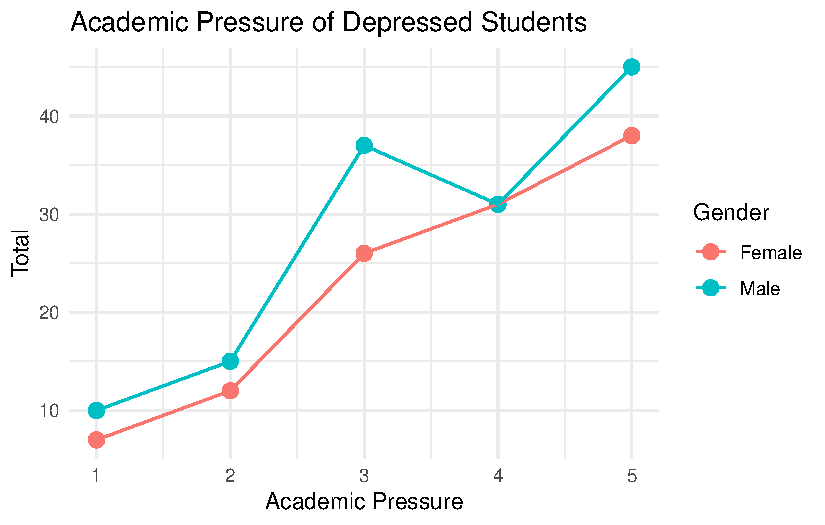
\includegraphics{Data_files/figure-pdf/unnamed-chunk-4-1.pdf}

\begin{Shaded}
\begin{Highlighting}[]
\FunctionTok{ggplot}\NormalTok{(are\_nd, }\FunctionTok{aes}\NormalTok{(}\AttributeTok{x =}\NormalTok{ Academic.Pressure, }\AttributeTok{y =}\NormalTok{ count, }\AttributeTok{color =}\NormalTok{ Gender)) }\SpecialCharTok{+}
  \FunctionTok{geom\_point}\NormalTok{(}\AttributeTok{size =} \DecValTok{3}\NormalTok{) }\SpecialCharTok{+}    
  \FunctionTok{geom\_line}\NormalTok{() }\SpecialCharTok{+}       
  \FunctionTok{labs}\NormalTok{(}
    \AttributeTok{title =} \StringTok{"Academic Pressure of Not Depressed Students"}\NormalTok{,}
    \AttributeTok{x =} \StringTok{"Academic Pressure"}\NormalTok{,}
    \AttributeTok{y =} \StringTok{"Total"}\NormalTok{,}
    \AttributeTok{color =} \StringTok{"Gender"}
\NormalTok{  ) }\SpecialCharTok{+}
  \FunctionTok{theme\_minimal}\NormalTok{() }
\end{Highlighting}
\end{Shaded}

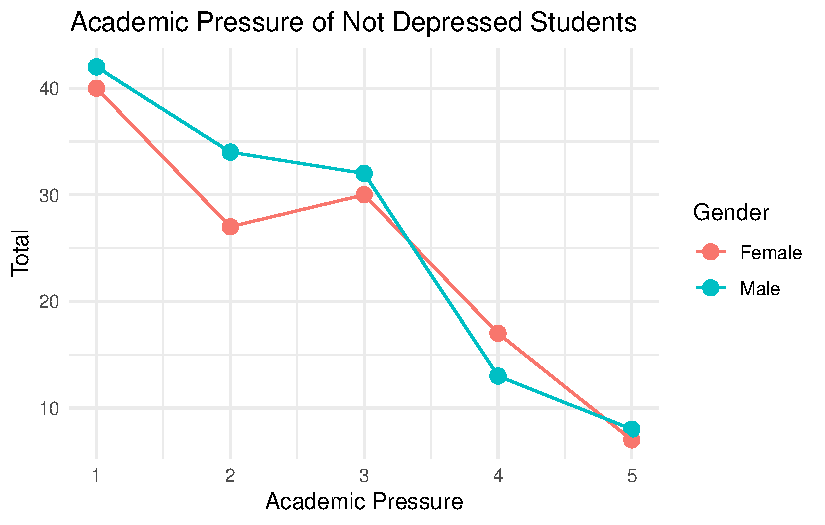
\includegraphics{Data_files/figure-pdf/unnamed-chunk-4-2.pdf}

\begin{Shaded}
\begin{Highlighting}[]
\NormalTok{depression\_study }\OtherTok{\textless{}{-}}\NormalTok{ depression }\SpecialCharTok{\%\textgreater{}\%} \FunctionTok{group\_by}\NormalTok{(Gender, Study.Satisfaction, Depression) }\SpecialCharTok{\%\textgreater{}\%} \FunctionTok{summarise}\NormalTok{(}\AttributeTok{count=}\FunctionTok{n}\NormalTok{())}
\end{Highlighting}
\end{Shaded}

\begin{verbatim}
`summarise()` has grouped output by 'Gender', 'Study.Satisfaction'. You can
override using the `.groups` argument.
\end{verbatim}

\begin{Shaded}
\begin{Highlighting}[]
\NormalTok{are\_d }\OtherTok{\textless{}{-}}\NormalTok{ depression\_study }\SpecialCharTok{\%\textgreater{}\%} \FunctionTok{filter}\NormalTok{(Depression }\SpecialCharTok{==} \StringTok{"Yes"}\NormalTok{)}
\NormalTok{are\_nd }\OtherTok{\textless{}{-}}\NormalTok{ depression\_study }\SpecialCharTok{\%\textgreater{}\%} \FunctionTok{filter}\NormalTok{(Depression }\SpecialCharTok{==} \StringTok{"No"}\NormalTok{)}

\FunctionTok{ggplot}\NormalTok{(are\_d, }\FunctionTok{aes}\NormalTok{(}\AttributeTok{x =}\NormalTok{ Study.Satisfaction, }\AttributeTok{y =}\NormalTok{ count, }\AttributeTok{color =}\NormalTok{ Gender)) }\SpecialCharTok{+}
  \FunctionTok{geom\_point}\NormalTok{(}\AttributeTok{size =} \DecValTok{3}\NormalTok{) }\SpecialCharTok{+}    
  \FunctionTok{geom\_line}\NormalTok{() }\SpecialCharTok{+}       
  \FunctionTok{labs}\NormalTok{(}
    \AttributeTok{title =} \StringTok{"Study Satisfaction of Depressed Students"}\NormalTok{,}
    \AttributeTok{x =} \StringTok{"Study Satisfaction"}\NormalTok{,}
    \AttributeTok{y =} \StringTok{"Total"}\NormalTok{,}
    \AttributeTok{color =} \StringTok{"Gender"}
\NormalTok{  ) }\SpecialCharTok{+}
  \FunctionTok{theme\_minimal}\NormalTok{() }
\end{Highlighting}
\end{Shaded}

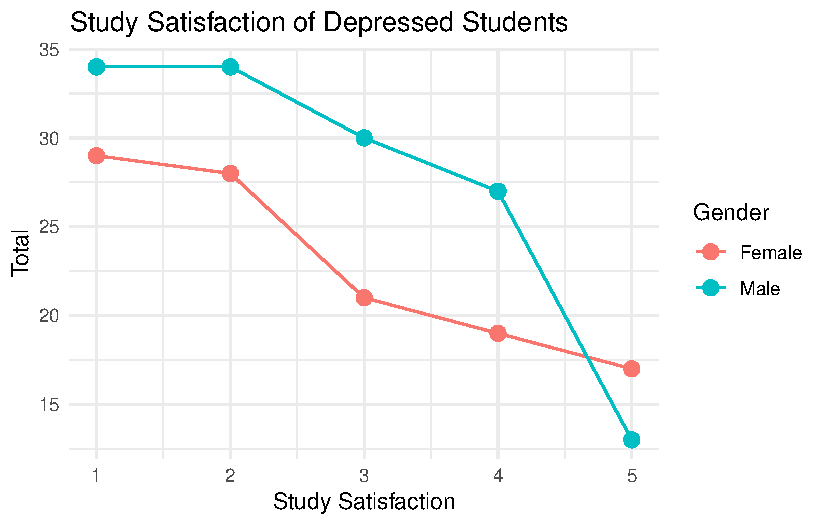
\includegraphics{Data_files/figure-pdf/unnamed-chunk-5-1.pdf}

\begin{Shaded}
\begin{Highlighting}[]
\FunctionTok{ggplot}\NormalTok{(are\_nd, }\FunctionTok{aes}\NormalTok{(}\AttributeTok{x =}\NormalTok{ Study.Satisfaction, }\AttributeTok{y =}\NormalTok{ count, }\AttributeTok{color =}\NormalTok{ Gender)) }\SpecialCharTok{+}
  \FunctionTok{geom\_point}\NormalTok{(}\AttributeTok{size =} \DecValTok{3}\NormalTok{) }\SpecialCharTok{+}    
  \FunctionTok{geom\_line}\NormalTok{() }\SpecialCharTok{+}       
  \FunctionTok{labs}\NormalTok{(}
    \AttributeTok{title =} \StringTok{"Study Satisfaction of Not Depressed Students"}\NormalTok{,}
    \AttributeTok{x =} \StringTok{"Study Satisfaction"}\NormalTok{,}
    \AttributeTok{y =} \StringTok{"Total"}\NormalTok{,}
    \AttributeTok{color =} \StringTok{"Gender"}
\NormalTok{  ) }\SpecialCharTok{+}
  \FunctionTok{theme\_minimal}\NormalTok{() }
\end{Highlighting}
\end{Shaded}

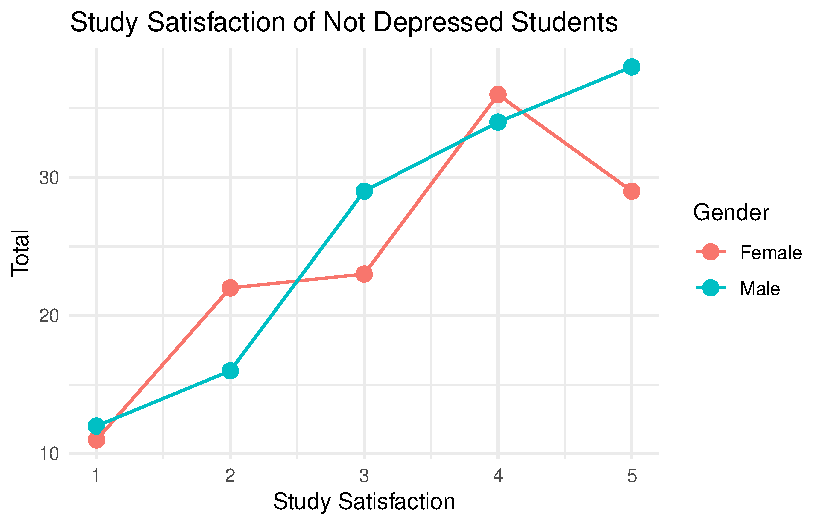
\includegraphics{Data_files/figure-pdf/unnamed-chunk-5-2.pdf}

\begin{Shaded}
\begin{Highlighting}[]
\NormalTok{depression\_sleep }\OtherTok{\textless{}{-}}\NormalTok{ depression }\SpecialCharTok{\%\textgreater{}\%} \FunctionTok{group\_by}\NormalTok{(Gender, Sleep.Duration, Depression) }\SpecialCharTok{\%\textgreater{}\%} \FunctionTok{summarise}\NormalTok{(}\AttributeTok{count=}\FunctionTok{n}\NormalTok{())}
\end{Highlighting}
\end{Shaded}

\begin{verbatim}
`summarise()` has grouped output by 'Gender', 'Sleep.Duration'. You can
override using the `.groups` argument.
\end{verbatim}

\begin{Shaded}
\begin{Highlighting}[]
\NormalTok{are\_d }\OtherTok{\textless{}{-}}\NormalTok{ depression\_sleep }\SpecialCharTok{\%\textgreater{}\%} \FunctionTok{filter}\NormalTok{(Depression }\SpecialCharTok{==} \StringTok{"Yes"}\NormalTok{)}
\NormalTok{are\_nd }\OtherTok{\textless{}{-}}\NormalTok{ depression\_sleep }\SpecialCharTok{\%\textgreater{}\%} \FunctionTok{filter}\NormalTok{(Depression }\SpecialCharTok{==} \StringTok{"No"}\NormalTok{)}

\FunctionTok{ggplot}\NormalTok{(are\_d, }\FunctionTok{aes}\NormalTok{(}\AttributeTok{x =}\NormalTok{ Sleep.Duration, }\AttributeTok{y =}\NormalTok{ count, }\AttributeTok{color =}\NormalTok{ Gender)) }\SpecialCharTok{+}
  \FunctionTok{geom\_point}\NormalTok{(}\AttributeTok{size =} \DecValTok{3}\NormalTok{) }\SpecialCharTok{+}    
  \FunctionTok{geom\_line}\NormalTok{() }\SpecialCharTok{+}       
  \FunctionTok{labs}\NormalTok{(}
    \AttributeTok{title =} \StringTok{"Sleep Duration of Depressed Students"}\NormalTok{,}
    \AttributeTok{x =} \StringTok{"Sleep Duration"}\NormalTok{,}
    \AttributeTok{y =} \StringTok{"Total"}\NormalTok{,}
    \AttributeTok{color =} \StringTok{"Gender"}
\NormalTok{  ) }\SpecialCharTok{+}
  \FunctionTok{theme\_minimal}\NormalTok{() }
\end{Highlighting}
\end{Shaded}

\begin{verbatim}
`geom_line()`: Each group consists of only one observation.
i Do you need to adjust the group aesthetic?
\end{verbatim}

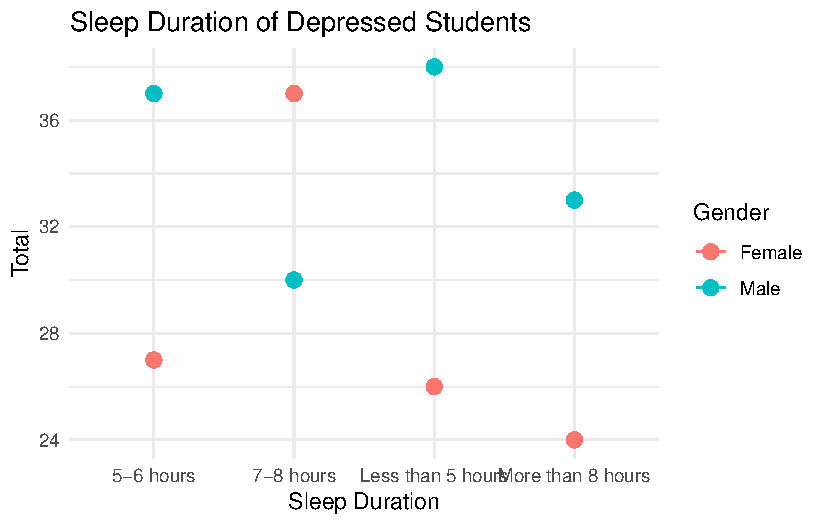
\includegraphics{Data_files/figure-pdf/unnamed-chunk-6-1.pdf}

\begin{Shaded}
\begin{Highlighting}[]
\FunctionTok{ggplot}\NormalTok{(are\_nd, }\FunctionTok{aes}\NormalTok{(}\AttributeTok{x =}\NormalTok{ Sleep.Duration, }\AttributeTok{y =}\NormalTok{ count, }\AttributeTok{color =}\NormalTok{ Gender)) }\SpecialCharTok{+}
  \FunctionTok{geom\_point}\NormalTok{(}\AttributeTok{size =} \DecValTok{3}\NormalTok{) }\SpecialCharTok{+}    
  \FunctionTok{geom\_line}\NormalTok{() }\SpecialCharTok{+}       
  \FunctionTok{labs}\NormalTok{(}
    \AttributeTok{title =} \StringTok{"Sleep Duration of Not Depressed Students"}\NormalTok{,}
    \AttributeTok{x =} \StringTok{"Sleep.Duration"}\NormalTok{,}
    \AttributeTok{y =} \StringTok{"Total"}\NormalTok{,}
    \AttributeTok{color =} \StringTok{"Gender"}
\NormalTok{  ) }\SpecialCharTok{+}
  \FunctionTok{theme\_minimal}\NormalTok{() }
\end{Highlighting}
\end{Shaded}

\begin{verbatim}
`geom_line()`: Each group consists of only one observation.
i Do you need to adjust the group aesthetic?
\end{verbatim}

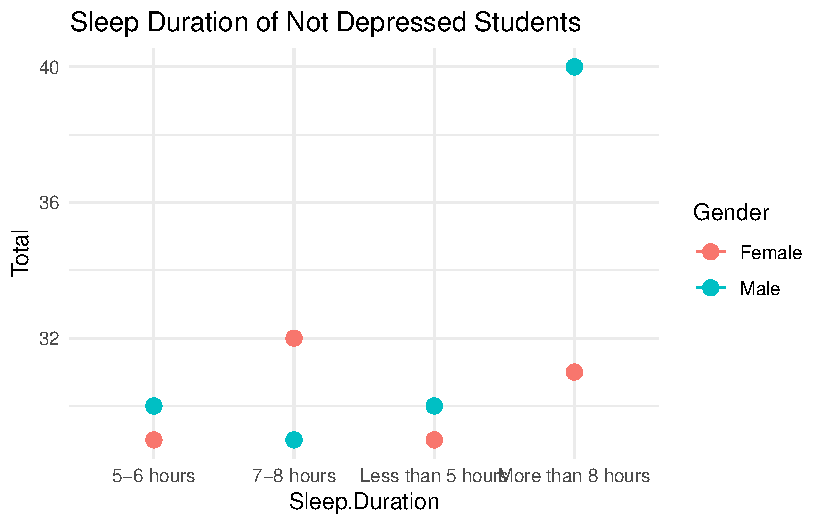
\includegraphics{Data_files/figure-pdf/unnamed-chunk-6-2.pdf}

\begin{Shaded}
\begin{Highlighting}[]
\NormalTok{depression\_diet }\OtherTok{\textless{}{-}}\NormalTok{ depression }\SpecialCharTok{\%\textgreater{}\%} \FunctionTok{group\_by}\NormalTok{(Gender, Dietary.Habits, Depression) }\SpecialCharTok{\%\textgreater{}\%} \FunctionTok{summarise}\NormalTok{(}\AttributeTok{count=}\FunctionTok{n}\NormalTok{())}
\end{Highlighting}
\end{Shaded}

\begin{verbatim}
`summarise()` has grouped output by 'Gender', 'Dietary.Habits'. You can
override using the `.groups` argument.
\end{verbatim}

\begin{Shaded}
\begin{Highlighting}[]
\NormalTok{are\_d }\OtherTok{\textless{}{-}}\NormalTok{ depression\_diet }\SpecialCharTok{\%\textgreater{}\%} \FunctionTok{filter}\NormalTok{(Depression }\SpecialCharTok{==} \StringTok{"Yes"}\NormalTok{)}
\NormalTok{are\_nd }\OtherTok{\textless{}{-}}\NormalTok{ depression\_diet }\SpecialCharTok{\%\textgreater{}\%} \FunctionTok{filter}\NormalTok{(Depression }\SpecialCharTok{==} \StringTok{"No"}\NormalTok{)}

\FunctionTok{ggplot}\NormalTok{(are\_d, }\FunctionTok{aes}\NormalTok{(}\AttributeTok{x =}\NormalTok{ Dietary.Habits, }\AttributeTok{y =}\NormalTok{ count, }\AttributeTok{color =}\NormalTok{ Gender)) }\SpecialCharTok{+}
  \FunctionTok{geom\_point}\NormalTok{(}\AttributeTok{size =} \DecValTok{3}\NormalTok{) }\SpecialCharTok{+}    
  \FunctionTok{geom\_line}\NormalTok{() }\SpecialCharTok{+}       
  \FunctionTok{labs}\NormalTok{(}
    \AttributeTok{title =} \StringTok{"Dietary Habits of Depressed Students"}\NormalTok{,}
    \AttributeTok{x =} \StringTok{"Dietary Habits"}\NormalTok{,}
    \AttributeTok{y =} \StringTok{"Total"}\NormalTok{,}
    \AttributeTok{color =} \StringTok{"Gender"}
\NormalTok{  ) }\SpecialCharTok{+}
  \FunctionTok{theme\_minimal}\NormalTok{() }
\end{Highlighting}
\end{Shaded}

\begin{verbatim}
`geom_line()`: Each group consists of only one observation.
i Do you need to adjust the group aesthetic?
\end{verbatim}

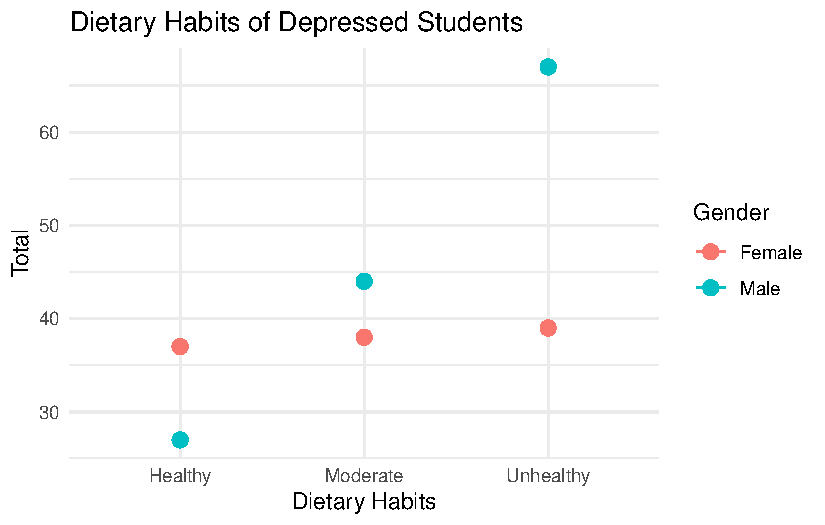
\includegraphics{Data_files/figure-pdf/unnamed-chunk-7-1.pdf}

\begin{Shaded}
\begin{Highlighting}[]
\FunctionTok{ggplot}\NormalTok{(are\_nd, }\FunctionTok{aes}\NormalTok{(}\AttributeTok{x =}\NormalTok{ Dietary.Habits, }\AttributeTok{y =}\NormalTok{ count, }\AttributeTok{color =}\NormalTok{ Gender)) }\SpecialCharTok{+}
  \FunctionTok{geom\_point}\NormalTok{(}\AttributeTok{size =} \DecValTok{3}\NormalTok{) }\SpecialCharTok{+}    
  \FunctionTok{geom\_line}\NormalTok{() }\SpecialCharTok{+}       
  \FunctionTok{labs}\NormalTok{(}
    \AttributeTok{title =} \StringTok{"Dietary Habits of Not Depressed Students"}\NormalTok{,}
    \AttributeTok{x =} \StringTok{"Dietary.Habits"}\NormalTok{,}
    \AttributeTok{y =} \StringTok{"Total"}\NormalTok{,}
    \AttributeTok{color =} \StringTok{"Gender"}
\NormalTok{  ) }\SpecialCharTok{+}
  \FunctionTok{theme\_minimal}\NormalTok{() }
\end{Highlighting}
\end{Shaded}

\begin{verbatim}
`geom_line()`: Each group consists of only one observation.
i Do you need to adjust the group aesthetic?
\end{verbatim}

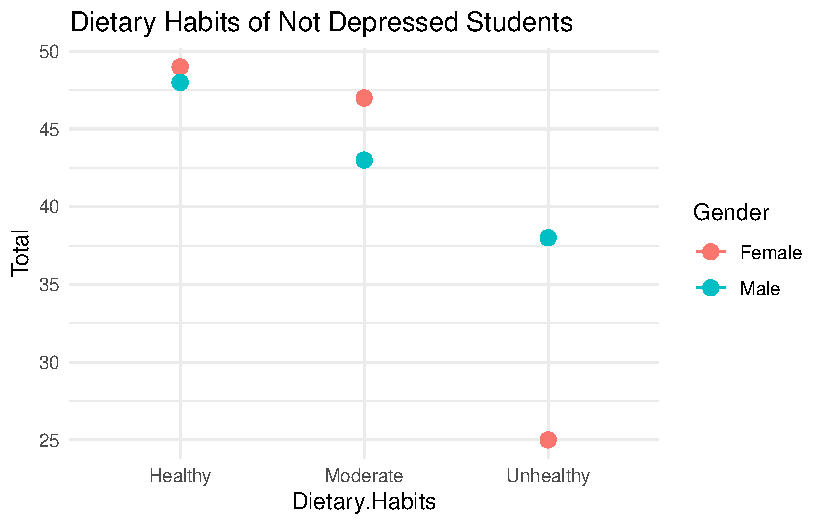
\includegraphics{Data_files/figure-pdf/unnamed-chunk-7-2.pdf}

\begin{Shaded}
\begin{Highlighting}[]
\NormalTok{depression\_suicidal }\OtherTok{\textless{}{-}}\NormalTok{ depression }\SpecialCharTok{\%\textgreater{}\%} \FunctionTok{group\_by}\NormalTok{(Gender, Have.you.ever.had.suicidal.thoughts.., Depression) }\SpecialCharTok{\%\textgreater{}\%} \FunctionTok{summarise}\NormalTok{(}\AttributeTok{count=}\FunctionTok{n}\NormalTok{())}
\end{Highlighting}
\end{Shaded}

\begin{verbatim}
`summarise()` has grouped output by 'Gender',
'Have.you.ever.had.suicidal.thoughts..'. You can override using the `.groups`
argument.
\end{verbatim}

\begin{Shaded}
\begin{Highlighting}[]
\NormalTok{are\_d }\OtherTok{\textless{}{-}}\NormalTok{ depression\_suicidal }\SpecialCharTok{\%\textgreater{}\%} \FunctionTok{filter}\NormalTok{(Depression }\SpecialCharTok{==} \StringTok{"Yes"}\NormalTok{)}
\NormalTok{are\_nd }\OtherTok{\textless{}{-}}\NormalTok{ depression\_suicidal }\SpecialCharTok{\%\textgreater{}\%} \FunctionTok{filter}\NormalTok{(Depression }\SpecialCharTok{==} \StringTok{"No"}\NormalTok{)}

\FunctionTok{ggplot}\NormalTok{(are\_d, }\FunctionTok{aes}\NormalTok{(}\AttributeTok{x =}\NormalTok{ Have.you.ever.had.suicidal.thoughts.., }\AttributeTok{y =}\NormalTok{ count, }\AttributeTok{color =}\NormalTok{ Gender)) }\SpecialCharTok{+}
  \FunctionTok{geom\_point}\NormalTok{(}\AttributeTok{size =} \DecValTok{3}\NormalTok{) }\SpecialCharTok{+}    
  \FunctionTok{geom\_line}\NormalTok{() }\SpecialCharTok{+}       
  \FunctionTok{labs}\NormalTok{(}
    \AttributeTok{title =} \StringTok{"Suicidal Thoughts vs Depression"}\NormalTok{,}
    \AttributeTok{x =} \StringTok{"Suicidal Thoughts"}\NormalTok{,}
    \AttributeTok{y =} \StringTok{"Total"}\NormalTok{,}
    \AttributeTok{color =} \StringTok{"Gender"}
\NormalTok{  ) }\SpecialCharTok{+}
  \FunctionTok{theme\_minimal}\NormalTok{() }
\end{Highlighting}
\end{Shaded}

\begin{verbatim}
`geom_line()`: Each group consists of only one observation.
i Do you need to adjust the group aesthetic?
\end{verbatim}

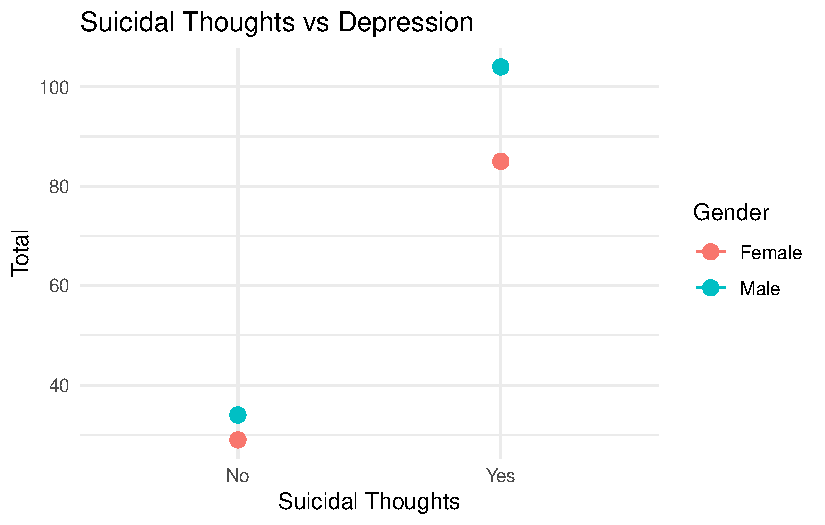
\includegraphics{Data_files/figure-pdf/unnamed-chunk-8-1.pdf}

\begin{Shaded}
\begin{Highlighting}[]
\FunctionTok{ggplot}\NormalTok{(are\_nd, }\FunctionTok{aes}\NormalTok{(}\AttributeTok{x =}\NormalTok{ Have.you.ever.had.suicidal.thoughts.., }\AttributeTok{y =}\NormalTok{ count, }\AttributeTok{color =}\NormalTok{ Gender)) }\SpecialCharTok{+}
  \FunctionTok{geom\_point}\NormalTok{(}\AttributeTok{size =} \DecValTok{3}\NormalTok{) }\SpecialCharTok{+}    
  \FunctionTok{geom\_line}\NormalTok{() }\SpecialCharTok{+}       
  \FunctionTok{labs}\NormalTok{(}
    \AttributeTok{title =} \StringTok{"Suicidal Thoughts vs No Depression"}\NormalTok{,}
    \AttributeTok{x =} \StringTok{"Suicidal Thoughts"}\NormalTok{,}
    \AttributeTok{y =} \StringTok{"Total"}\NormalTok{,}
    \AttributeTok{color =} \StringTok{"Gender"}
\NormalTok{  ) }\SpecialCharTok{+}
  \FunctionTok{theme\_minimal}\NormalTok{() }
\end{Highlighting}
\end{Shaded}

\begin{verbatim}
`geom_line()`: Each group consists of only one observation.
i Do you need to adjust the group aesthetic?
\end{verbatim}

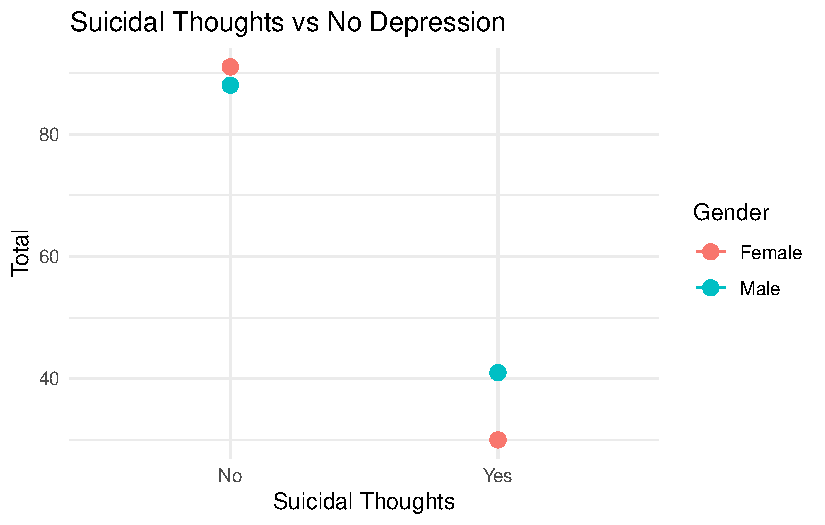
\includegraphics{Data_files/figure-pdf/unnamed-chunk-8-2.pdf}

\begin{Shaded}
\begin{Highlighting}[]
\NormalTok{depression\_study\_h }\OtherTok{\textless{}{-}}\NormalTok{ depression }\SpecialCharTok{\%\textgreater{}\%} \FunctionTok{group\_by}\NormalTok{(Gender, Study.Hours, Depression) }\SpecialCharTok{\%\textgreater{}\%} \FunctionTok{summarise}\NormalTok{(}\AttributeTok{count=}\FunctionTok{n}\NormalTok{())}
\end{Highlighting}
\end{Shaded}

\begin{verbatim}
`summarise()` has grouped output by 'Gender', 'Study.Hours'. You can override
using the `.groups` argument.
\end{verbatim}

\begin{Shaded}
\begin{Highlighting}[]
\NormalTok{are\_d }\OtherTok{\textless{}{-}}\NormalTok{ depression\_study\_h }\SpecialCharTok{\%\textgreater{}\%} \FunctionTok{filter}\NormalTok{(Depression }\SpecialCharTok{==} \StringTok{"Yes"}\NormalTok{)}
\NormalTok{are\_nd }\OtherTok{\textless{}{-}}\NormalTok{ depression\_study\_h }\SpecialCharTok{\%\textgreater{}\%} \FunctionTok{filter}\NormalTok{(Depression }\SpecialCharTok{==} \StringTok{"No"}\NormalTok{)}

\FunctionTok{ggplot}\NormalTok{(are\_d, }\FunctionTok{aes}\NormalTok{(}\AttributeTok{x =}\NormalTok{ Study.Hours, }\AttributeTok{y =}\NormalTok{ count, }\AttributeTok{color =}\NormalTok{ Gender)) }\SpecialCharTok{+}
  \FunctionTok{geom\_point}\NormalTok{(}\AttributeTok{size =} \DecValTok{3}\NormalTok{) }\SpecialCharTok{+}    
  \FunctionTok{geom\_line}\NormalTok{() }\SpecialCharTok{+}       
  \FunctionTok{labs}\NormalTok{(}
    \AttributeTok{title =} \StringTok{"Study Hours of Depressed Students"}\NormalTok{,}
    \AttributeTok{x =} \StringTok{"Study Hours"}\NormalTok{,}
    \AttributeTok{y =} \StringTok{"Total"}\NormalTok{,}
    \AttributeTok{color =} \StringTok{"Gender"}
\NormalTok{  ) }\SpecialCharTok{+}
  \FunctionTok{theme\_minimal}\NormalTok{() }
\end{Highlighting}
\end{Shaded}

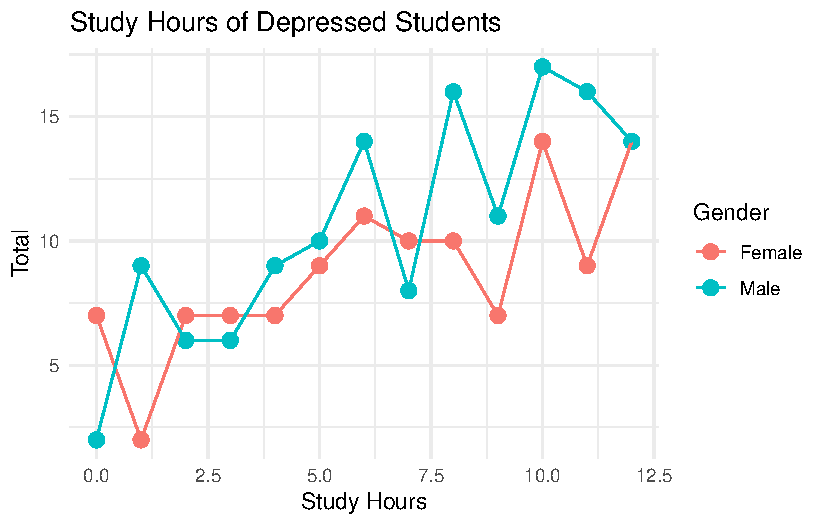
\includegraphics{Data_files/figure-pdf/unnamed-chunk-9-1.pdf}

\begin{Shaded}
\begin{Highlighting}[]
\FunctionTok{ggplot}\NormalTok{(are\_nd, }\FunctionTok{aes}\NormalTok{(}\AttributeTok{x =}\NormalTok{ Study.Hours, }\AttributeTok{y =}\NormalTok{ count, }\AttributeTok{color =}\NormalTok{ Gender)) }\SpecialCharTok{+}
  \FunctionTok{geom\_point}\NormalTok{(}\AttributeTok{size =} \DecValTok{3}\NormalTok{) }\SpecialCharTok{+}    
  \FunctionTok{geom\_line}\NormalTok{() }\SpecialCharTok{+}       
  \FunctionTok{labs}\NormalTok{(}
    \AttributeTok{title =} \StringTok{"Study Hours of Not Depressed Students"}\NormalTok{,}
    \AttributeTok{x =} \StringTok{"Study Hours"}\NormalTok{,}
    \AttributeTok{y =} \StringTok{"Total"}\NormalTok{,}
    \AttributeTok{color =} \StringTok{"Gender"}
\NormalTok{  ) }\SpecialCharTok{+}
  \FunctionTok{theme\_minimal}\NormalTok{() }
\end{Highlighting}
\end{Shaded}

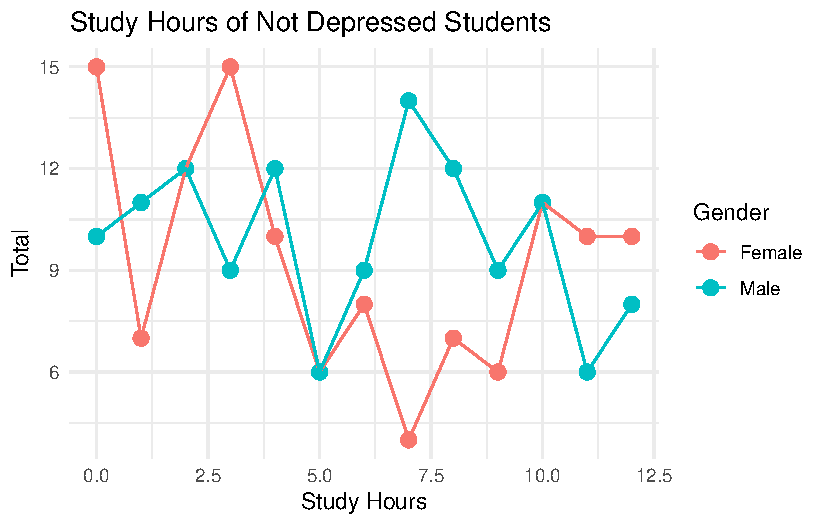
\includegraphics{Data_files/figure-pdf/unnamed-chunk-9-2.pdf}

\begin{Shaded}
\begin{Highlighting}[]
\NormalTok{depression\_finance }\OtherTok{\textless{}{-}}\NormalTok{ depression }\SpecialCharTok{\%\textgreater{}\%} \FunctionTok{group\_by}\NormalTok{(Gender, Financial.Stress, Depression) }\SpecialCharTok{\%\textgreater{}\%} \FunctionTok{summarise}\NormalTok{(}\AttributeTok{count=}\FunctionTok{n}\NormalTok{())}
\end{Highlighting}
\end{Shaded}

\begin{verbatim}
`summarise()` has grouped output by 'Gender', 'Financial.Stress'. You can
override using the `.groups` argument.
\end{verbatim}

\begin{Shaded}
\begin{Highlighting}[]
\NormalTok{are\_d }\OtherTok{\textless{}{-}}\NormalTok{ depression\_finance }\SpecialCharTok{\%\textgreater{}\%} \FunctionTok{filter}\NormalTok{(Depression }\SpecialCharTok{==} \StringTok{"Yes"}\NormalTok{)}
\NormalTok{are\_nd }\OtherTok{\textless{}{-}}\NormalTok{ depression\_finance }\SpecialCharTok{\%\textgreater{}\%} \FunctionTok{filter}\NormalTok{(Depression }\SpecialCharTok{==} \StringTok{"No"}\NormalTok{)}

\FunctionTok{ggplot}\NormalTok{(are\_d, }\FunctionTok{aes}\NormalTok{(}\AttributeTok{x =}\NormalTok{ Financial.Stress, }\AttributeTok{y =}\NormalTok{ count, }\AttributeTok{color =}\NormalTok{ Gender)) }\SpecialCharTok{+}
  \FunctionTok{geom\_point}\NormalTok{(}\AttributeTok{size =} \DecValTok{3}\NormalTok{) }\SpecialCharTok{+}    
  \FunctionTok{geom\_line}\NormalTok{() }\SpecialCharTok{+}       
  \FunctionTok{labs}\NormalTok{(}
    \AttributeTok{title =} \StringTok{"Financial Stress of Depressed Students"}\NormalTok{,}
    \AttributeTok{x =} \StringTok{"Financial Stress"}\NormalTok{,}
    \AttributeTok{y =} \StringTok{"Total"}\NormalTok{,}
    \AttributeTok{color =} \StringTok{"Gender"}
\NormalTok{  ) }\SpecialCharTok{+}
  \FunctionTok{theme\_minimal}\NormalTok{() }
\end{Highlighting}
\end{Shaded}

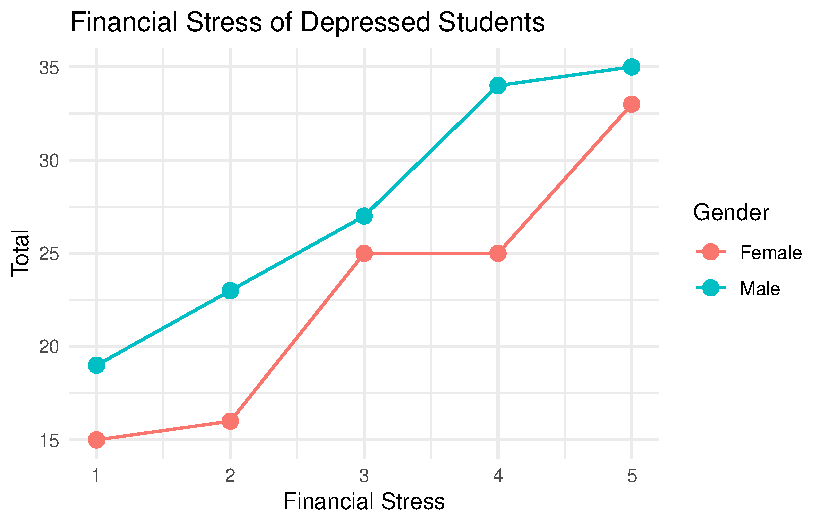
\includegraphics{Data_files/figure-pdf/unnamed-chunk-10-1.pdf}

\begin{Shaded}
\begin{Highlighting}[]
\FunctionTok{ggplot}\NormalTok{(are\_nd, }\FunctionTok{aes}\NormalTok{(}\AttributeTok{x =}\NormalTok{ Financial.Stress, }\AttributeTok{y =}\NormalTok{ count, }\AttributeTok{color =}\NormalTok{ Gender)) }\SpecialCharTok{+}
  \FunctionTok{geom\_point}\NormalTok{(}\AttributeTok{size =} \DecValTok{3}\NormalTok{) }\SpecialCharTok{+}    
  \FunctionTok{geom\_line}\NormalTok{() }\SpecialCharTok{+}       
  \FunctionTok{labs}\NormalTok{(}
    \AttributeTok{title =} \StringTok{"Financial Stress of Not Depressed Students"}\NormalTok{,}
    \AttributeTok{x =} \StringTok{"Financial Stress"}\NormalTok{,}
    \AttributeTok{y =} \StringTok{"Total"}\NormalTok{,}
    \AttributeTok{color =} \StringTok{"Gender"}
\NormalTok{  ) }\SpecialCharTok{+}
  \FunctionTok{theme\_minimal}\NormalTok{() }
\end{Highlighting}
\end{Shaded}

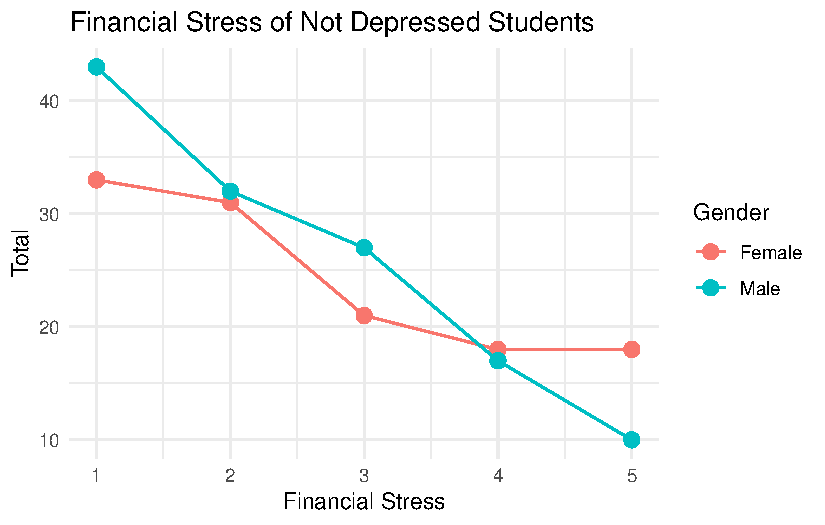
\includegraphics{Data_files/figure-pdf/unnamed-chunk-10-2.pdf}

\begin{Shaded}
\begin{Highlighting}[]
\NormalTok{depression\_fam }\OtherTok{\textless{}{-}}\NormalTok{ depression }\SpecialCharTok{\%\textgreater{}\%} \FunctionTok{group\_by}\NormalTok{(Gender, Family.History.of.Mental.Illness, Depression) }\SpecialCharTok{\%\textgreater{}\%} \FunctionTok{summarise}\NormalTok{(}\AttributeTok{count=}\FunctionTok{n}\NormalTok{())}
\end{Highlighting}
\end{Shaded}

\begin{verbatim}
`summarise()` has grouped output by 'Gender',
'Family.History.of.Mental.Illness'. You can override using the `.groups`
argument.
\end{verbatim}

\begin{Shaded}
\begin{Highlighting}[]
\NormalTok{are\_d }\OtherTok{\textless{}{-}}\NormalTok{ depression\_fam }\SpecialCharTok{\%\textgreater{}\%} \FunctionTok{filter}\NormalTok{(Depression }\SpecialCharTok{==} \StringTok{"Yes"}\NormalTok{)}
\NormalTok{are\_nd }\OtherTok{\textless{}{-}}\NormalTok{ depression\_fam }\SpecialCharTok{\%\textgreater{}\%} \FunctionTok{filter}\NormalTok{(Depression }\SpecialCharTok{==} \StringTok{"No"}\NormalTok{)}

\FunctionTok{ggplot}\NormalTok{(are\_d, }\FunctionTok{aes}\NormalTok{(}\AttributeTok{x =}\NormalTok{ Family.History.of.Mental.Illness, }\AttributeTok{y =}\NormalTok{ count, }\AttributeTok{color =}\NormalTok{ Gender)) }\SpecialCharTok{+}
  \FunctionTok{geom\_point}\NormalTok{(}\AttributeTok{size =} \DecValTok{3}\NormalTok{) }\SpecialCharTok{+}    
  \FunctionTok{geom\_line}\NormalTok{() }\SpecialCharTok{+}       
  \FunctionTok{labs}\NormalTok{(}
    \AttributeTok{title =} \StringTok{"Family History of Mental Illness of Depressed Students"}\NormalTok{,}
    \AttributeTok{x =} \StringTok{"Family History of Mental Illness"}\NormalTok{,}
    \AttributeTok{y =} \StringTok{"Total"}\NormalTok{,}
    \AttributeTok{color =} \StringTok{"Gender"}
\NormalTok{  ) }\SpecialCharTok{+}
  \FunctionTok{theme\_minimal}\NormalTok{() }
\end{Highlighting}
\end{Shaded}

\begin{verbatim}
`geom_line()`: Each group consists of only one observation.
i Do you need to adjust the group aesthetic?
\end{verbatim}

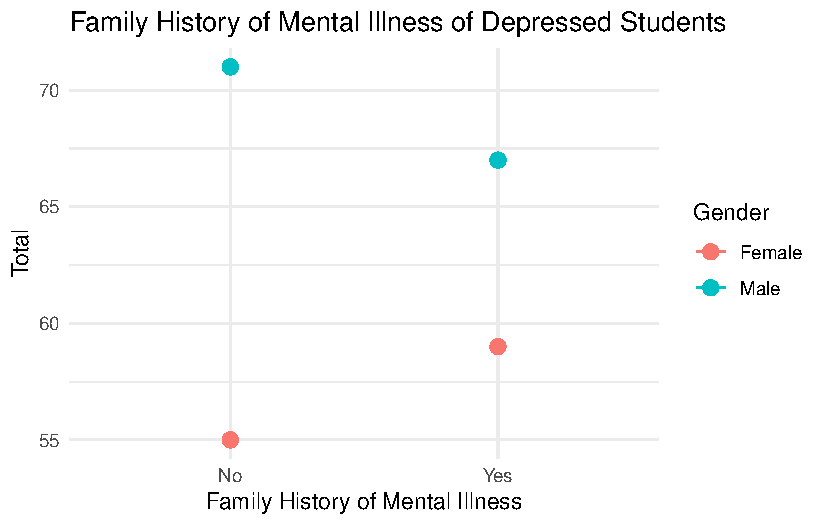
\includegraphics{Data_files/figure-pdf/unnamed-chunk-11-1.pdf}

\begin{Shaded}
\begin{Highlighting}[]
\FunctionTok{ggplot}\NormalTok{(are\_nd, }\FunctionTok{aes}\NormalTok{(}\AttributeTok{x =}\NormalTok{ Family.History.of.Mental.Illness, }\AttributeTok{y =}\NormalTok{ count, }\AttributeTok{color =}\NormalTok{ Gender)) }\SpecialCharTok{+}
  \FunctionTok{geom\_point}\NormalTok{(}\AttributeTok{size =} \DecValTok{3}\NormalTok{) }\SpecialCharTok{+}    
  \FunctionTok{geom\_line}\NormalTok{() }\SpecialCharTok{+}       
  \FunctionTok{labs}\NormalTok{(}
    \AttributeTok{title =} \StringTok{"Family History of Mental Illness of Not Depressed Students"}\NormalTok{,}
    \AttributeTok{x =} \StringTok{"Family History of Mental Illness"}\NormalTok{,}
    \AttributeTok{y =} \StringTok{"Total"}\NormalTok{,}
    \AttributeTok{color =} \StringTok{"Gender"}
\NormalTok{  ) }\SpecialCharTok{+}
  \FunctionTok{theme\_minimal}\NormalTok{() }
\end{Highlighting}
\end{Shaded}

\begin{verbatim}
`geom_line()`: Each group consists of only one observation.
i Do you need to adjust the group aesthetic?
\end{verbatim}

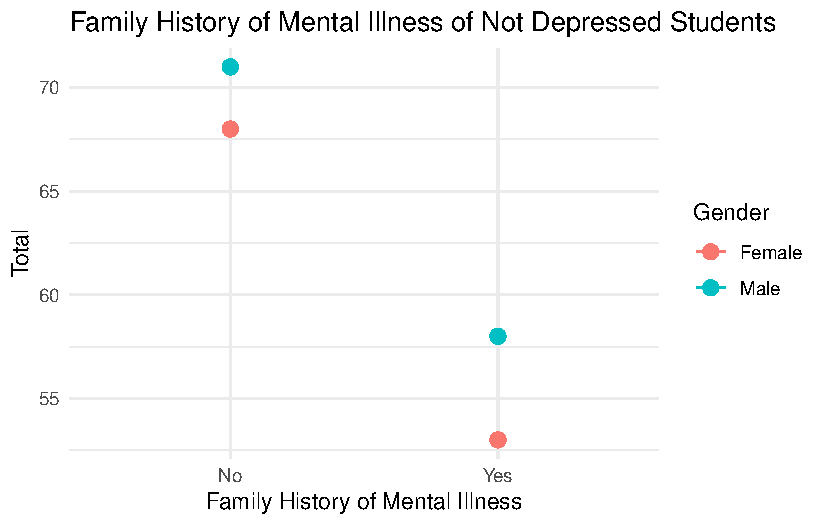
\includegraphics{Data_files/figure-pdf/unnamed-chunk-11-2.pdf}

\begin{Shaded}
\begin{Highlighting}[]
\NormalTok{depression\_is\_depressed }\OtherTok{\textless{}{-}}\NormalTok{ depression }\SpecialCharTok{\%\textgreater{}\%} \FunctionTok{group\_by}\NormalTok{(Gender, Depression) }\SpecialCharTok{\%\textgreater{}\%} \FunctionTok{summarise}\NormalTok{(}\AttributeTok{count=}\FunctionTok{n}\NormalTok{())}
\end{Highlighting}
\end{Shaded}

\begin{verbatim}
`summarise()` has grouped output by 'Gender'. You can override using the
`.groups` argument.
\end{verbatim}

The \texttt{echo:\ false} option disables the printing of code (only
output is displayed).




\end{document}
